\documentclass[journal]{IEEEtran}
\usepackage[utf8]{inputenc}
\usepackage{graphicx}
\usepackage{amsmath}
\usepackage{siunitx}
\usepackage{xspace}
\usepackage{hyperref}
\usepackage{url}
\usepackage{cite}
\hyphenation{op-tical net-works semi-conduc-tor}

\begin{document}
	
	\title{Laboratorio 3: Lógica combinacional y Aritmética I}
	\author{Fiorella, Jonathan, Gerald}
	\date{Marzo 2021}
	
	\newcommand{\email}[1]{\href{mailto:#1}{#1}}
	
	\author{
		\IEEEauthorblockN
		{
			Fiorella Delgado León
			Jonathan Guzmán Araya,
			Gerald Valverde McKenzie
		}
		\IEEEauthorblockA{\\Instituto Tecnológico de Costa Rica}
		\IEEEauthorblockA{\\Área Académica Ingeniería en Computadores}
		
		\IEEEauthorblockA{\email{fio@gmail.com}}		
		\IEEEauthorblockA{\email{jonathana1196@gmail.com}}
		\IEEEauthorblockA{\email{gerald@gmail.com}}
	}
	
	% The paper headers
	\markboth{Laboratorio Taller de Diseño Digital, Semestre I~2021}%
	{Shell \MakeLowercase{\textit{et al.}}: Bare Demo of IEEEtran.cls for IEEE Journals}
	
	
	% make the title area
	\maketitle
	
	% As a general rule, do not put math, special symbols or citations
	% in the abstract or keywords.
	\begin{abstract}

	\end{abstract}
	% Note that keywords are not normally used for peerreview papers.
	\begin{IEEEkeywords}
		ALU, compuertas lógicas, flip-flops, microprocesadores
	\end{IEEEkeywords}
	
	\section{Introducción}	
	Los circuitos combinacionales son aquellos en los que las salidas solo dependen solamente de las entradas, y no de ningún tipo de sincronización con señales de reloj, esto hace que los sistemas combinacionales sean generalmente rápidos. En sistemas digitales complejos, como los microprocesadores, los circuitos de lógica combinacional desempeñan un papel fundamental. La arquitectura de un microprocesador es como la que se observa en la Figura \ref{fig:microprocesador}.
	
	\begin{figure}[hbtp]
		\centering
		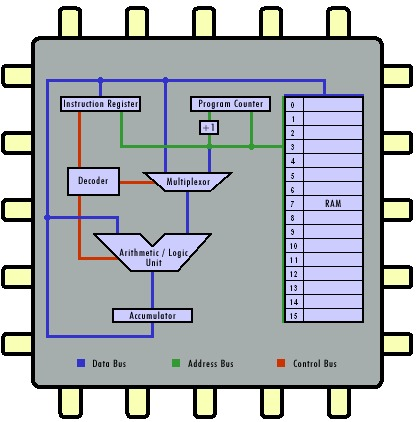
\includegraphics[scale = 0.5]{img/microprocesador.jpg}
		\caption{Arquitectura básica de un microprocesador \cite{Gonzalez2017}}
		\label{fig:microprocesador}
	\end{figure}
	
	Una función esencial de muchas computadoras (microprocesadores) y calculadoras es la realización de operaciones lógicas y aritméticas. Estas operaciones se efectúan en la unidad aritmética-lógica de una computadora, donde se combinan compuertas lógicas y flip-flops de manera que puedan sumar, restar, multiplicar y dividir números binarios \cite{Tocci2007}. El símbolo de una ALU es como el de la Figura \ref{fig:simboloalu}.
	
	\begin{figure}[!htb]
		\centering
		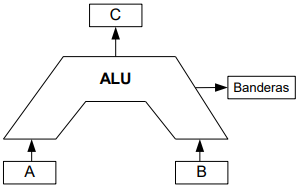
\includegraphics[scale = 0.5]{img/simboloalu.png}
		\caption{Símbolo ALU \cite{Garcia}}
		\label{fig:simboloalu}
	\end{figure}
	
	Además de los operadores lógicos, la ALU cuenta con una serie de registros para almacenar los datos y bits de información sobre los resultados, también llamados banderas \cite{Garcia}, las banderas más comunes en una ALU son: $Z$, $C$, $V$, $N$.
	\begin{itemize}
		\item Zero flag: usada para determinar si dos valores son iguales, generalmente se usa una resta, y se revisa si el resultado es cero, si es así, esta bandera se enciende.
		\item Overflow flag: usada para determinar si el resultado de una operación (usualmente suma o multiplicación), tiene un tamaño superior al máximo representable, o inferior al mínimo representable en la ALU, es posible que existan como banderas separadas.
		\item Negative flag: usada para determinar si el resultado de una resta es menor a cero
		\item Carry/Borrow flag: Esta bandera indica cuando una operación  resulta en un valor más largo del cual el acumulador puede representar o menor del cual el acumulador puede representar.
	\end{itemize}
	
	La ALU es simplemente un operador, es decir solo realiza operaciones, esta no toma decisiones, acepta datos binarios que están almacenados en la memoria y ejecuta operaciones con estos datos, de acuerdo a las instrucciones que vienen de la unidad de control.
	
	Para realizar operaciones lógicas la ALU utiliza compuertas lógicas como:
	
	\begin{itemize}
		\item NOT: La Figura \ref{fig:NOT} muestra el símbolo para un circuito NOT, la operación NOT cambia de un nivel lógico al nivel lógico opuesto. Cuando la entrada está a nivel ALTO (1), la salida se pone a nivel BAJO (0). Cuando la entrada está a nivel BAJO, la salida se pone a nivel ALTO \cite{Floyd2006}.
		
		\begin{figure}
			\centering
			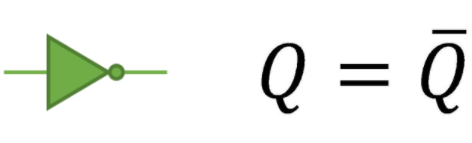
\includegraphics[scale = 0.5]{img/NOT.png}
			\caption{Compuerta NOT y su representación en álgebra de Boole \cite{Tocci2007}}
			\label{fig:NOT}
		\end{figure}
		
		\begin{table}[!htb]
			\centering
			\begin{tabular}{|c|c|}
				\hline
				Q & Q' \\
				\hline
				\hline
				0 & 1 \\
				\hline
				1 & 0 \\
				\hline
			\end{tabular}
			\caption{Tabla de verdad de la compuerta NOT}
			\label{tab:NOT}
		\end{table}
		
		\item AND: La Figura \ref{fig:AND} muestra el símbolo lógico para una compuerta AND de dos entradas. La operación AND genera un nivel ALTO sólo cuando todas las entradas están a nivel ALTO, para el caso de dos entradas. Cuando una entrada está a nivel ALTO y la otra entrada está a nivel ALTO, la salida se pone a nivel ALTO. Cuando cualquiera de las entradas o todas ellas están a nivel BAJO, la salida se pone a nivel BAJO \cite{Floyd2006}.
		
		\begin{figure}[!htb]
			\centering
			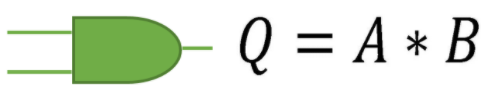
\includegraphics[scale = 0.3]{img/AND.png}
			\caption{Compuerta AND y su representación en álgebra de Boole \cite{Tocci2007}}
			\label{fig:AND}
		\end{figure}
		
		\begin{table}[!htb]
			\centering
			\begin{tabular}{|c|c|c|}
				\hline
				A & B & Q \\
				\hline
				\hline
				0 & 0 & 0 \\
				\hline
				0 & 1 & 0 \\
				\hline
				1 & 0 & 0 \\
				\hline
				1 & 1 & 1 \\
				\hline
			\end{tabular}
			\caption{Tabla de verdad de la compuerta AND}
			\label{tab:AND}
		\end{table}
		
		\item OR: La Figura \ref{fig:OR} muestra el símbolo lógico para una compuerta OR de dos entradas. La operación OR genera un nivel ALTO cuando una o más entradas están a nivel ALTO, para el caso de dos entradas. Cuando una de las entradas está a nivel ALTO o ambas entradas
		están a nivel ALTO, la salida es un nivel ALTO. Cuando ambas entradas están a nivel BAJO, la salida será un nivel BAJO \cite{Floyd2006}.
		
		\begin{figure}[!htb]
			\centering
			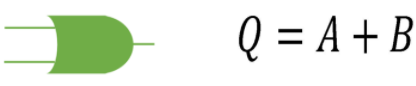
\includegraphics[scale = 0.35]{img/OR.png}
			\caption{Compuerta OR y su representación en álgebra de Boole \cite{Tocci2007}}
			\label{fig:OR}
		\end{figure}
		
		\begin{table}[!htb]
			\centering
			\begin{tabular}{|c|c|c|}
				\hline
				A & B & Q \\
				\hline
				\hline
				0 & 0 & 0 \\
				\hline
				0 & 1 & 1 \\
				\hline
				1 & 0 & 1 \\
				\hline
				1 & 1 & 1 \\
				\hline
			\end{tabular}
			\caption{Tabla de verdad de la compuerta OR}
			\label{tab:OR}
		\end{table}
		
		\item XOR: La Figura \ref{fig:XOR} muestra el símbolo lógico para una compuerta XOR de dos entradas. En una compuerta OR-exclusiva, la salida X es un nivel ALTO si la entrada A está a nivel BAJO y la entrada B está a nivel ALTO; o si la entrada A está a nivel ALTO y la entrada B está a nivel BAJO; X es un nivel BAJO si tanto A como B están a nivel ALTO o BAJO \cite{Floyd2006}.
		
		\begin{figure}[!htb]
			\centering
			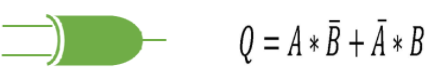
\includegraphics[scale = 0.4]{img/XOR.png}
			\caption{Compuerta XOR y su representación en álgebra de Boole \cite{Tocci2007}}
			\label{fig:XOR}
		\end{figure}
		
		\begin{table}[!htb]
			\centering
			\begin{tabular}{|c|c|c|}
				\hline
				A & B & Q \\
				\hline
				\hline
				0 & 0 & 0 \\
				\hline
				0 & 1 & 1 \\
				\hline
				1 & 0 & 1 \\
				\hline
				1 & 1 & 0 \\
				\hline
			\end{tabular}
			\caption{Tabla de verdad de la compuerta XOR}
			\label{tab:XOR}
		\end{table}
	\end{itemize}
	
	
	
	Uno de los problemas más desafiantes en el diseño de circuitos es el tiempo, hacer que un circuito funcione rápido. Una salida necesita tiempo para cambiar en respuesta a un cambio en la entrada, como se observa en la Figura \ref{fit:delay} \cite{SarahL.Harris2010}.
	
	\begin{figure}[hbtp]
		\centering
		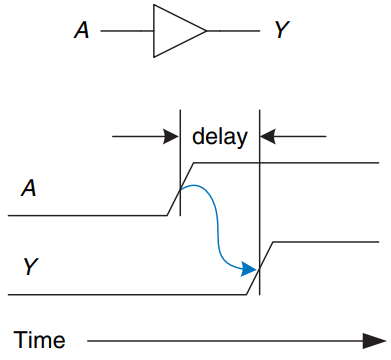
\includegraphics[scale = 0.4]{img/delay.png}
		\caption{Tiempo de respuesta de una señal \cite{SarahL.Harris2010}}
		\label{fit:delay}
	\end{figure}

	En la lógica combinacional existen dos tipos de tiempos, tiempo de propagación y tiempo de contaminación. El tiempo de propagación $t_{pd}$ es el tiempo máximo desde que la entrada cambia hasta que el o las salidas llegan a su valor final y el tiempo de contaminación $t_{cd}$ es el tiempo mínimo que dura la entrada en cambiar hasta que alguna salida empiece a cambiar su valor \cite{SarahL.Harris2010}.
	
	Además de los tiempos de propagación y contaminación en la electrónica de circuitos existe algo llamado la ruta crítica, que es la ruta más larga que tiene una entrada, hablando de circuitos combinacionales, para llegar a la salida, por lo tanto, esta ruta también sería la más lenta. Ahora para describir a un circuito hay dos factores muy importantes: latencia y tasa de transferencia. La latencia funcionaria como la frecuencia del circuito, ya que es el tiempo que se necesita para que el cambio en la entrada haga un cambio en la salida; esta puede ser expresada en tiempo o, para circuitos sincrónicos, un cierto número de ciclos de reloj.  Y la tasa de transferencia a la velocidad con la que la información puede ser procesada. Por ejemplo, en la Figura \ref{fig:criticalpath} se tienen tres rutas distintas desde una entrada hasta la salida, siendo la ruta azul la más lenta de estas.
	
	\begin{figure}[hbtp]
		\centering
		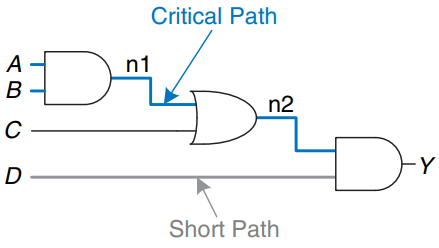
\includegraphics[scale = 0.4]{img/criticalpath.png}
		\caption{Ruta crítica \cite{SarahL.Harris2010}}
		\label{fig:criticalpath}
	\end{figure}

	Así el tiempo de propagación de un circuito combinacional es la suma de los tiempos de propagación de cada elemento que lo compone como se observa en la Ecuación \ref{eq:tpd} y el tiempo de contaminación es la suma de los tiempos de contaminación de la más corta del circuito combinacional que se puede observar en la Ecuación \ref{eq:tcd}.
	
	\begin{equation}
		t_{pd} = 2t_{pdAND} + t_{pdOR}
		%\caption{Tiempo de propagación del circuito}
		\label{eq:tpd}
	\end{equation}

	\begin{equation}
		t_{pd} = 2t_{pdAND} + t_{pdOR}
		%\caption{Tiempo de contaminación del circuito}
		\label{eq:tcd}
	\end{equation}

	En circuitos más complejos como un procesador pipeline como el de la Figura \ref{fig:pipe}, la velocidad de ciclos del reloj decrece haciendo retrasos en la ruta crítica, para esto se utiliza la técnica de Pipelining, el cual consiste en dividir el circuito en varias partes con un registro al final de cada una, de esta manera se divide la ruta crítica en pequeñas rutas, permitiendo que la velocidad del reloj aumente y consecuentemente también lo haga la tasa de transferencia. La segmentación consiste en descomponer la ejecución de cada instrucción en varias etapas para poder empezar a procesar una instrucción diferente en cada una de ellas y trabajar con varias a la vez. Las etapas de segmentación pueden ser: IF (búsqueda), ID (decodificación), EX (ejecución), MEM (memoria), WB (escritura), en una arquitectura relativamente sencilla.
	
	\begin{figure}[hbtp]
		\centering
		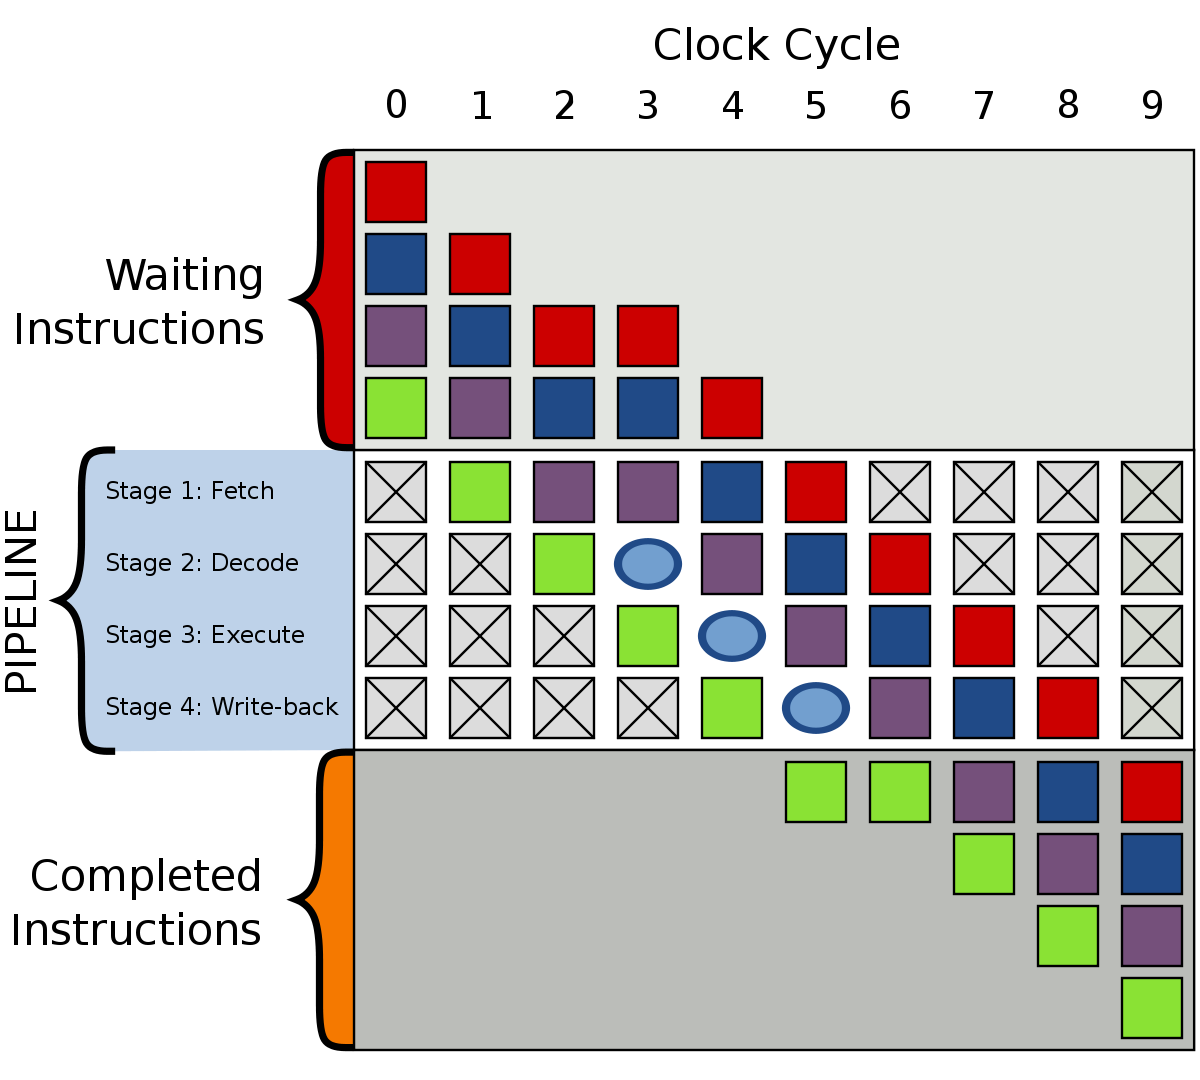
\includegraphics[scale = 0.15]{img/Pipe.jpg}
		\caption{Procesador Pipeline \cite{pipewiki}}
		\label{fig:pipe}
	\end{figure}

	La frecuencia máxima de operación de un circuito está determinada por la ruta crítica del mismo, para esto se toma la ruta crítica (en un procesador se realiza tomando la instrucción que tarda más en ejecutarse por completo sin afectar a las otras) y se calcula el tiempo que tarda en ciclos de reloj $T_{c}$, como se observa en la Ecuación \ref{eq:fHz}, esta frecuencia se mide en $Hz$.
	
	\begin{equation}
		f_{c} = \dfrac{1}{T_{c}}
		%\caption{Frecuencia de un circuito}
		\label{eq:fHz}
	\end{equation}
	
	\section{Conclusiones}
	
	\section{Bibliografía}
	
	\bibliographystyle{IEEEtran}
	\bibliography{myref}
	
\end{document}